\ifx\wholebook\relax\else
\input{../Common.tex}
\input{../macroes.tex}
\begin{document}
\fi

\project
\chapter{Simple L-Systems and Fractal Production}\label{ch:lsystem}

\begin{chapterfigure}
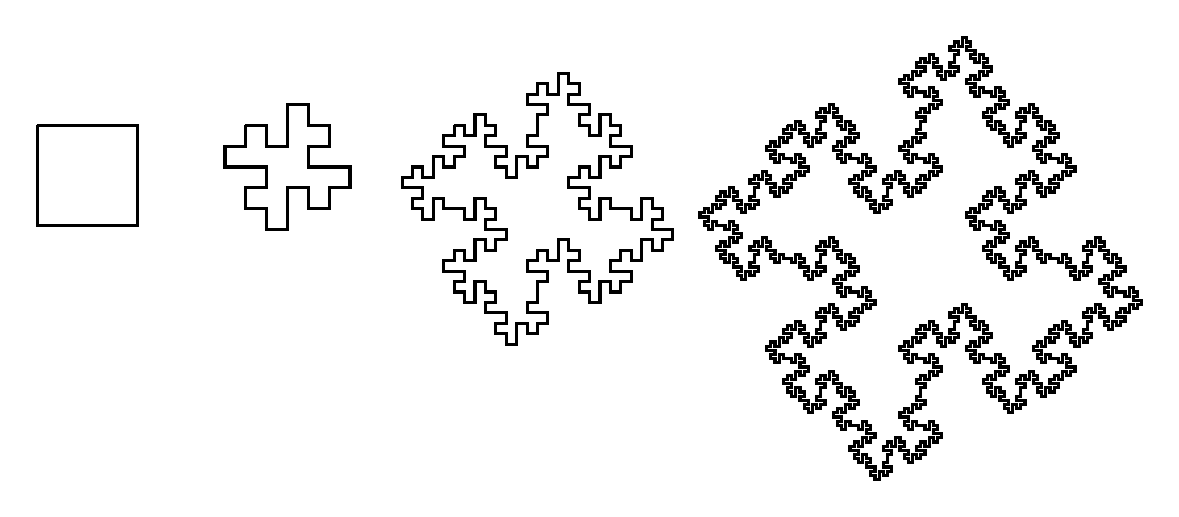
\includegraphics[width=\linewidth]{drawallKoch}
\end{chapterfigure}


Aristide Lindermayer worked on the understanding and representation of
plant growth. He invented a way to describe how simple plants and algua grow. 
This approach is named L-Systems. Although L-Systems are used 
to describe the plant growth, they can also be applied to produce fractal
graphics \--- graphics based on repetitions of themselves, as the ones above.  Moreover, the graphical interpretation of L-Systems is easy with a turtle. This is
what we explore in this chapter. In this chapter, we propose you to implement 
the simplest form of L-System.


\section{L-Systems}\label{sec:lsystem}
L-Systems is a generic term of designing different rule-based
rewriting systems. A rewriting rule-based system is a system that
given an \emph{input} like a sequence of characters, strings, or
numbers and the \emph{set of rules} explaining how an element of the
input is replaced by new ones, produces an \emph{output}. 

\begin{figure}
\begin{center}
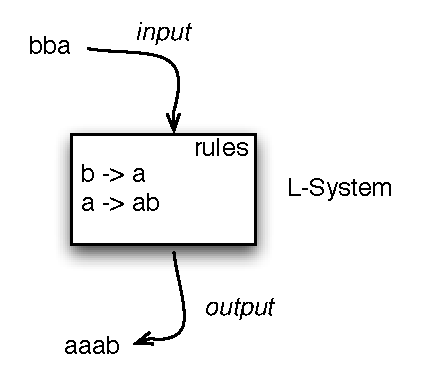
\includegraphics{inputOutput}
\label{An L-System is composed of: a set of rules. It takes an input and produces an output in which the rules have been applied on the input.}
\end{center}
\end{figure}

Let us look at the simple example\footnote{A fun aspect of this L-System
is that the length of the production is the Fibonacci suite.} below. 

\begin{tabbing}
\=aaa\=aaa\=aaa\=aaa\=aaa\=aaa\=aaa\=aaa\=aaa\kill
Fibonacci \\
\>\>\emph{Rule 1: b $\rightarrow$ a}\\
\>\>\emph{Rule 2: a $\rightarrow$ a b}
\end{tabbing}

It is composed by two rules, the first means that every $b$ has to
be replaced by an $a$, the second means that every $a$ has to the
replaced by $ab$. Now if we start with $b$ and apply the two rules
we obtain the following results where each line represents the
application of the rules to the result of the previous line.

\begin{tabbing}
\=aaa\=aaa\=aaa\=aaaaaaaaa\=aaaaaaaaa\=aaaaaaaaa\=aaaaaaaaa\=aaaaaaaaa\=aaaaaaaaa\kill
\>\>\>\> \emph{Input} \>\> \emph{b}\\
\>\>\>\> \emph{(Rule 1)} \>\> $\rightarrow$ \emph{a }\\
\>\>\>\> \emph{(Rule 2)} \>\> $\rightarrow$ \emph{a b}  \\
\>\>\>\> \emph{(Rules 2, 1)} \>\> $\rightarrow$  \emph{a b a}  \\
\>\>\>\> \emph{(Rules 2, 1, 2)} \>\>$\rightarrow$ \emph{a b a a b}  \\
\>\>\>\> \emph{(Rules 2, 1, 2, 2, 1)} \>\>$\rightarrow$ \emph{a b a a b a b a} 
\end{tabbing}

We call the first \emph{input}, in the example \emph{b}, the \emph{original input} of the L-System. Note that we say that we \emph{apply} a rule. We call the symbols $a$ and $b$ that constitutes the first input and output the vocabulary of the L-System.

\paragraph{Analysis.}
Let us analyse this simple L-System\footnote{Certain L-Systems are
much more complex and take into account the context of the element or
some other parameters before applying the rule.} and understand the
basic mechanisms used here:

\begin{itemize}
\item An L-System can contain several rules. Here we have two rules namely
Rule 1 that transforms every element $b$ into $a$ and Rule 2 that
transforms every $a$ into the sequence of elements $a b$. 

\item A rule is composed by two parts: a \emph{left} and a \emph{right} 
part.  The left part identifies the element in the input that will be
replaced by the right part. The left part
of a rule only identifies \emph{one} element while the right part can
be \emph{one or multiple} elements.
  
\item \emph{Applying a rule} means replacing in the current
input the element (left part of the rule) by the sequence of elements
described in the right part of the rule. For example, the third line
above is produced by applying the Rule 1 and substituing $a$ by $a b$.

\item The rules are applied each time they can be applied.   For example, the production of the fourth line is the result of
applying the Rule 2 and the Rule 1 to the sequence $a b$.  Note that
the application order is irrevelant as long as it is performed in
parallel \ie that a rule is only applied on the input and not on the result of another rule application.

\item A rule can be applied several times.  The production of the last line is the result of the application of the rules 2, 1, 2, 2 and 1.

\item The input does not have to be necessary one single element. 

\end{itemize}

%\paragraph{Parallel or Sequential Rule Application.} 
%In computer science, language grammars are often described using
%rewiting rule based like systems. However, the production of an
%L-System is the result of the \strong{parallel} application of the
%rules, whereas in language grammar rules are applied in
%\emph{sequence}, only one rule at during one iteration. The reason is
%that both systems are not used to model similar concept. L-Systems
%parallel rule application is adapted to represent the parallel growth
%of plant cellula, while grammars are used to represent choice or paths
%to follow.






%%%%%%%%%%%%%%%%%%%%%%%%%%%%%%%%%%%%%%%%%%%%%%%%%%%%%%%%%%%%%
\section{The Graphical Interpretation of L-Systems}
Besides representing plant growth, L-Systems are also interesting
systems because we can use them to produce graphics representing
plants or fractals. Fractals are graphics that are built using
repetitive patterns and that also partially or fully contain
themselves. The idea to produce such graphics based on L-Systems is to use L-System whose vocabulary is mapped to turtle actions. 

\subsection{A Turtle Dialect for L-Systems}
To produce graphics we chose to define the vocabulary of the L-Systems  the following way: input and rules only manipulate a limited set of predefined symbols representing turtle methods. These symbols are:

\begin{itemize}
\item[\ct{F}]: the turtle goes forward and leaves a trace from a given distance. 
It corresponds to  our \go method.

\item[\ct{f}]: the turtle goes forward without leaving a trace from a given distance. It corresponds to our \jump method.

\item[\ct{+}]: the turtle turns on the left from a given angle. 
It corresponds to our \turnLeft method.

\item[\ct{-}]: the turtle turns on the right from a given angle. 
It corresponds to our \turnRight method.
\end{itemize}

This simplest form of L-System are based on an angle and a length to
move forward that are defined \emph{once} for all the rules of the
L-System. The value of these data does not change during the rules
application or graphical interpretation. This is the reason why you
have to pay attention of the length we define if we want to have
reasonable output. 

\subsection{A First L-System based on Turtle Actions}

\begin{figure}
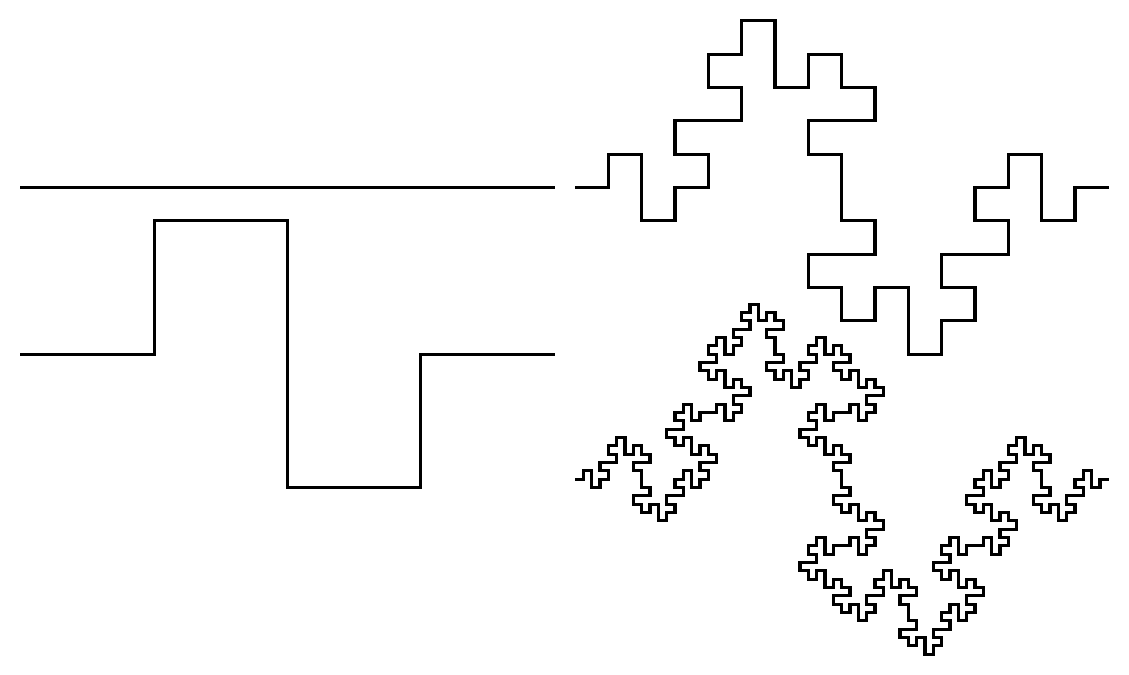
\includegraphics[width=\linewidth]{drawallN}
\caption{Steps 0, 1, 2 and 3 of the L-System defined by Input: F, Angle=90, F $\rightarrow$ F+F-F-FF+F+F-F. As a segment is cut into 4 segments, we divide the length by 4 from iteration to iteration. The lengths of the picture are 64 * 4, 64, 16 and 4.}\label{fig:nsteps}
\end{figure}

Let us look at the following example whose first application steps are
illustrated by Figure~\ref{fig:nsteps}.

\begin{tabbing}
\=aaa\=aaa\=aaa\=aaaaaaaaa\=aaaaaaaaa\=aaaaaaaaa\=aaaaaaaaa\=aaaaaaaaa\=aaaaaaaaa\kill
Figure~\ref{fig:nsteps}\\
\>\>\>\> \emph{Input} \>\>\emph{F}\\
\>\>\>\> \emph{Angle} \>\>90 degree\\
\>\>\>\> \emph{Rule}  \>\>\emph{F $\rightarrow$ F+F-F-FF+F+F-F}
\end{tabbing}

\begin{itemize}
\item The input represents the geometrical shape that we take as starting point. Here \emph{F} means that we start with a line, \emph{F+F+F+F} a square as the angle is 90 degree.

\item The rule describes how one segment is transformed in the second steps of Figure~\ref{fig:nsteps}.
\end{itemize}

Applying several times the rule produces the other graphics shown in
Figure~\ref{fig:nsteps}. Figure~\ref{fig:n1n2} superposes two
graphics on the same picture to show how the rule application
decomposes the segments into smaller ones.


\begin{figure}
\center{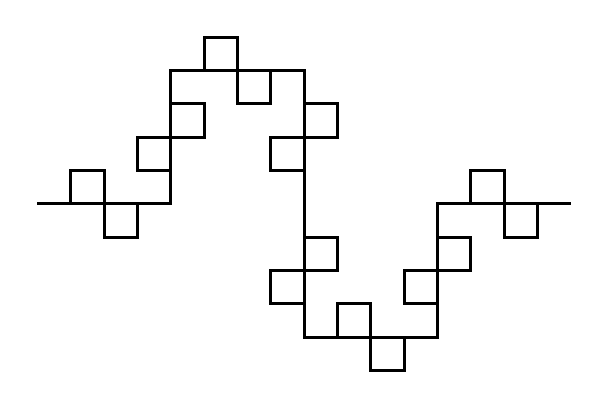
\includegraphics{drawallTwoN}}
\caption{The superposition of the graphics produced after the second iteration and after the third iteration shows how the previous figure is decomposed.}\label{fig:n1n2}
\end{figure}


Pay attention that applying the rules at the different levels can become really quickly huge output. For example here are the results of this L-System  for the level application steps : 
\begin{itemize}
\item \emph{0 $\rightarrow$ F}, 
\item  \emph{1 $\rightarrow$
F+F-F-FF+F+F-F},
\item \emph{ 2 $\rightarrow$
F+F-F-FF+F+F-F+F+F-F-FF+F+F-F-F+F-F-FF+F+F-F-F+F-F-FF+F+F-FF+F-F-FF+F+F-F+F+F-F-FF+F+F-F+F+F-F-FF+F+F-F-F+F-F-FF+F+F-F},
\item \emph{3 $\rightarrow$
F+F-F-FF+F+F-F+F+F-F-FF+F+F-F-F+F-F-FF+F+F-F-F+F-F-FF+F+F-FF+F-F-FF+F+F-F+F+F-F
-FF+F+F-F+F+F-F-FF+F+F-F-F+F-F-FF+F+F-F+F+F-F-FF+F+F-F+F+F-F-FF+F+F-F-F+F-F-FF+F+F-F-F+F-F-FF+F+F-FF+F-F-FF+F+F-F+F+F-F-FF+F+F-F+F+F-F-FF+F+F-F-F+F-F-FF+F+F-F-F+F-F-FF+F+F-F+F+F-F-FF+F+F-F-F+F-F-FF+F+F-F-F+F-F-FF+F+F-FF+F-F-FF+F+F-F+F+F-F-FF+F+F-F+F+F-F-FF+F+F-F-F+F-F-FF+F+F-F-F+F-F-FF+F+F-F+F+F-F-FF+F+F-F-F+F-F-FF+F+F-F-F+F-F-FF+F+F-FF+F-F-FF+F+F-F+F+F-F-FF+F+F-F+F+F-F-FF+F+F-F-F+F-F-FF+F+F-FF+F-F-FF+F+F-F+F+F-F-FF+F+F-F-F+F-F-FF+F+F-F-F+F-F-FF+F+F-FF+F-F-FF+F+F-F+F+F-F-FF+F+F-F+F+F-F-FF+F+F-F-F+F-F-FF+F+F-F+F+F-F-FF+F+F-F+F+F-F-FF+F+F-F-F+F-F-FF+F+F-F-F+F-F-FF+F+F-FF+F-F-FF+F+F-F+F+F-F-FF+F+F-F+F+F-F-FF+F+F-F-F+F-F-FF+F+F-F+F+F-F-FF+F+F-F+F+F-F-FF+F+F-F-F+F-F-FF+F+F-F-F+F-F-FF+F+F-FF+F-F-FF+F+F-F+F+F-F-FF+F+F-F+F+F-F-FF+F+F-F-F+F-F-FF+F+F-F-F+F-F-FF+F+F-F+F+F-F-FF+F+F-F-F+F-F-FF+F+F-F-F+F-F-FF+F+F-FF+F-F-FF+F+F-F+F+F-F-FF+F+F-F+F+F-F-FF+F+F-F-F+F-F-FF+F+F-F}
\end{itemize}

So take care during your experimentation not to ask crazy numbers, you
could think that the system is down but it would be just computing for
hours. Finally we could have used directly the name of the turtle methods but this would have led to overly long L-System definitions. Moreover, we prefer to stick with the original L-System notation.

\section{Implementing the L-System}
As shown in Chapter~\ref{cha:condition} it is easy to add
functionality to the class \ct{Turtle} so that turtles are able to
interpret a string composed by the L-System symbols F, f, +, and - and
perform the corresponding actions. You should remember that a string
is a collection of characters and that characters are single letter
beginning with \$. Simple L-Systems defines \emph{once} for all the length of which a turtle should go forward and the angle they should turn. So define the method \ct{interpretChar: aChar length: len angle: degree} that sends the action described by \ct{aChar} to the receiver turtle. If the character is \ct{\$F} or \ct{\$f} the turtle should go
forward (with trace and without trace) from \ct{len} distance. If the
character is \ct{\$+} or \ct{\$-} the turtle receiver should
respectively to the left or right from \ct{degree}. The \scriptref{scr:anU} should draw an U. A possible solution is shown in the method~\ref{mth:interpretSymb}. 

\begin{scriptwithouttitle}\label{scr:anU}
|aTurtle|
aTurtle := Turtle new.
aTurtle interpretChar: \$F length: 100 angle: 90.
aTurtle interpretChar: \$+ length: 100 angle: 90.
aTurtle interpretChar: \$F length: 100 angle: 90.
aTurtle interpretChar: \$+ length: 100 angle: 90.
aTurtle interpretChar: \$f length: 100 angle: 90.
aTurtle interpretChar: \$+ length: 100 angle: 90.
aTurtle interpretChar: \$F length: 100 angle: 90.
\end{scriptwithouttitle}




\begin{method}\cat{L-System}\label{mth:interpretSymb}
interpretChar: aChar length: len angle: degree 
      
   aChar = \$F
      ifTrue: [self go: len]
      ifFalse: [aChar = \$+
                    ifTrue: [self turnLeft: degree]
                    ifFalse: [aChar = \$- 
                                  ifTrue: [self turnRight: degree]
                                  ifFalse: [aChar =\$f
                                               ifTrue: [self jump: len]]]
\end{method}




Now we want to treat \emph{sequences} of characters and not characters one by one. Therefore define the method \ct{interpret: aCollection length: len angle: degree} that knows how to interpret a string, \ie a collection of characters. Hints: String is a subclass of Collection so operations available on collections such as \ct{do:} are also possible on strings. The \scriptref{scr:anUM} should also draw an U.
\begin{scriptwithouttitle}\label{scr:anUM}
|aTurtle|
aTurtle := Turtle new.
aTurtle interpret: 'F+F+f+F' length: 100 angle: 90.
\end{scriptwithouttitle}

A possible solution is shown in method~\ref{mth:inter}

\begin{method}\cat{L-System}\label{mth:inter}
interpret: aString length: len angle: degree
    aString do: [:each | self interpretChar: each length: len angle: degree]
\end{method}

Now we are ready to implement the application of rules on an input. 

\section{L-Systems with a Single Loops}
For now we limit our approach to the simplest L-System: a system
containing only one rule. We took this decision so that you
could have a fast idea of the process. What is missing now is the application of the rule on an input. We want to be able to specify an input, the rule to apply, a number of times the rule should be applied.  Define the
method \ct{applyOnInput: aString leftPart: leftPart rightPart: rightPart level: n}.  Just remember that computing the input a certain number of time requires to apply any possible rules then reiterate the rule application on the result you obtained previously.
To help you, the method \ct{copyReplaceAll:with:} defined on
the class \ct{SequenceCollection} replaces all the occurences of a string by another in the receiver as shown by the script~\ref{scr:replaceall}.


\begin{scriptwithouttitle}\label{scr:replaceall}
'How now brown cow?' copyReplaceAll: 'ow' with: 'ello'
\pr 'Hello nello brellon cello?'
\end{scriptwithouttitle}

\begin{scriptwithouttitle}
|aTurtle|
aTurtle := Turtle new.
aTurtle applyOnInput: 'F' leftPart: 'F' rightPart: 'F+F-F-FF+F+F-F' level: 1
\pr'F+F-F-FF+F+F-F'
aTurtle applyOnInput: 'F' leftPart: 'F' rightPart: 'F+F-F-FF+F+F-F' level: 0
\pr 'F'
aTurtle applyOnInput: 'F' leftPart: 'F' rightPart: 'F+F-F-FF+F+F-F' level: 2
\pr 'F+F-F-FF+F+F-F+F+F-F-FF+F+F-F-F+F-F-FF+F+F-F-F+F-F-\\ FF+F+F-FF+F-F-FF+F+F-F+F+F-F-FF+F+F-F+F+F-F-FF+F+F-F-F+F-F-FF+F+F-F'
\end{scriptwithouttitle}

Here is a possible implementation of the method \ct{applyOnInput:leftPart:rightPart:level:} is shown in the method definition~\ref{mth:apply}.

\begin{method}\cat{L-System}\label{mth:apply}
applyOnInput: input leftPart: start rightPart: repl level: n
   "Generate the nth output of a simple L-System composed of one rule
   replacing leftPart by rightPart in input"
       
   |production|
   production := input.
   n timesRepeat: [production := self 
                                   replace: start
                                   by: repl 
                                   in: production].
   \^ production
\end{method}

\begin{method}
replace: aCharacter by: aCollection in: aSequence 
   \^ aSequence copyReplaceAll: aCharacter with: aCollection
\end{method}

Now you are in the position to produce your first graphics. You have
to use the methods \ct{applyOnInput:leftPart:rightPart:level:} and
\ct{interpret:length:angle:}. Try to program the L-System we show previously. 

\begin{tabbing}
\=aaa\=aaa\=aaa\=aaaaaaaaa\=aaaaaaaaa\=aaaaaaaaa\=aaaaaaaaa\=aaaaaaaaa\=aaaaaaaaa\kill
Figure~\ref{fig:nsteps}\\
\>\>\>\> \emph{Input} \>\>\emph{F}\\
\>\>\>\> \emph{Angle} \>\>90 degree\\
\>\>\>\> \emph{Rule}  \>\>\emph{F $\rightarrow$ F+F-F-FF+F+F-F}
\end{tabbing}



\section{A Gallery of 1-rule based L-Systems}
We show you some of the pictures that you can now create. The first pictures of this chapter are generated by the following L-System. This family of curves are called Koch curves. The other pictures of this chapter are generated using the described L-Systems. Note that some of them may take some time to draw.

\begin{tabbing}
\=aaa\=aaa\=aaaaaaa\=aaaaaaaaa\=aaaaaaaaa\=aaaaaaaaa\=aaaaaaaaa\=aaaaaaaaa\=aaaaaaaaa\kill
First Pictures of the Chapter \\
\>\> \emph{Input} \>\>\emph{F-F-F-F}\\
\>\> \emph{Angle} \>\>90 degree\\
\>\> \emph{Rule}  \>\>\emph{F $\rightarrow$ F-F+F+FF-F-F+F}
\end{tabbing}

\begin{figure}[!h]
\centerline{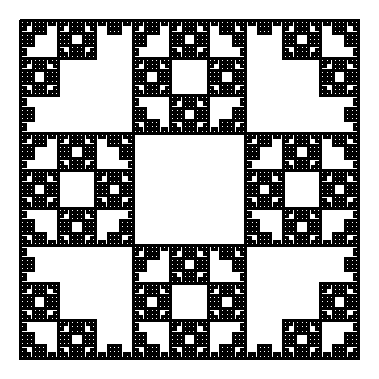
\includegraphics{LSsystemKochb}}
\caption{Variation on Koch curve 2: n = 4, angle = 90, Input: \emph{F-F-F-F}, \emph{F $\rightarrow$ FF-F-F-F-FF}}
\label{fig:Kochb}
\end{figure}

\begin{tabbing}
\=aaa\=aaa\=aaaaaaa\=aaaaaaaaa\=aaaaaaaaa\=aaaaaaaaa\=aaaaaaaaa\=aaaaaaaaa\=aaaaaaaaa\kill
Figure~\ref{fig:Kochb} \\
\>\> \emph{Input} \>\>\emph{F-F-F-F}\\
\>\> \emph{Angle} \>\>90 degree\\
\>\> \emph{Rule}  \>\>\emph{F $\rightarrow$ FF-F-F-F-FF}
\end{tabbing}


\begin{figure}[!h]
\centerline{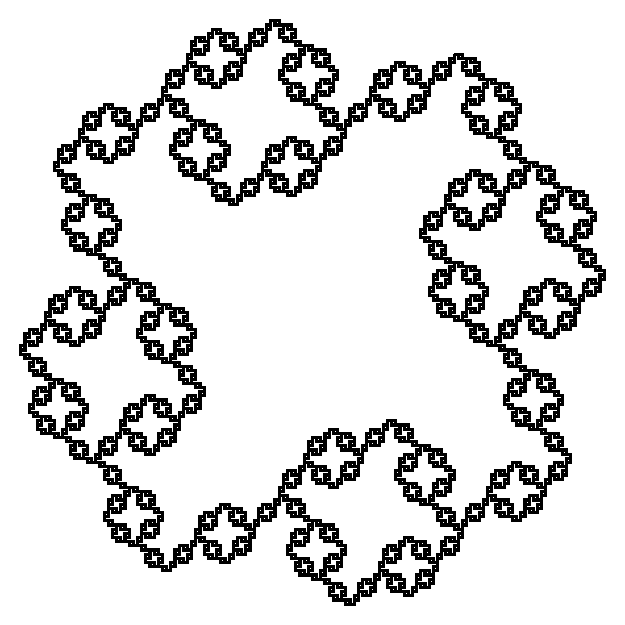
\includegraphics[width=8cm]{LSsystemKocha}}
\caption{Variation on Koch curve 1: n = 4, angle = 90, Input: \emph{F-F-F-F}, \emph{F $\rightarrow$ FF-F-F-F-F-F+F}}
\label{fig:Kocha}
\end{figure}


\begin{tabbing}
\=aaa\=aaa\=aaaaaa\=aaaaaaaaa\=aaaaaaaaa\=aaaaaaaaa\=aaaaaaaaa\=aaaaaaaaa\=aaaaaaaaa\kill
Figure~\ref{fig:Kocha} \\
\>\> \emph{Input} \>\>\emph{F-F-F-F}\\
\>\> \emph{Angle} \>\>90 degree\\
\>\> \emph{Rule}  \>\>\emph{F $\rightarrow$ FF-F-F-F-F-F+F}
\end{tabbing}






\begin{figure}[!htbp]
\centerline{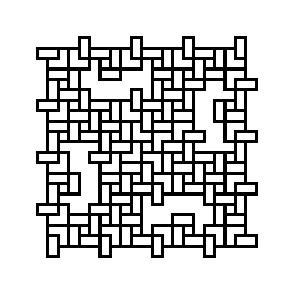
\includegraphics{LSsystemKochc}}
\caption{Variation on Koch curve 3: n = 3, angle = 90, Input: \emph{F-F-F-F}, \emph{F $\rightarrow$ FF-F-F+F-F-FF}}
\label{fig:Kochc}
\end{figure}

\begin{tabbing}
\=aaa\=aaa\=aaaaaa\=aaaaaaaaa\=aaaaaaaaa\=aaaaaaaaa\=aaaaaaaaa\=aaaaaaaaa\=aaaaaaaaa\kill
Figure~\ref{fig:Kochc} \\
\>\> \emph{Input} \>\>\emph{'F-F-F-F'}\\
\>\> \emph{Angle} \>\>90 degree\\
\>\> \emph{Rule}  \>\>\emph{F $\rightarrow$ FF-F+F-F-FF}
\end{tabbing}


\begin{figure}[!htbp]
\centerline{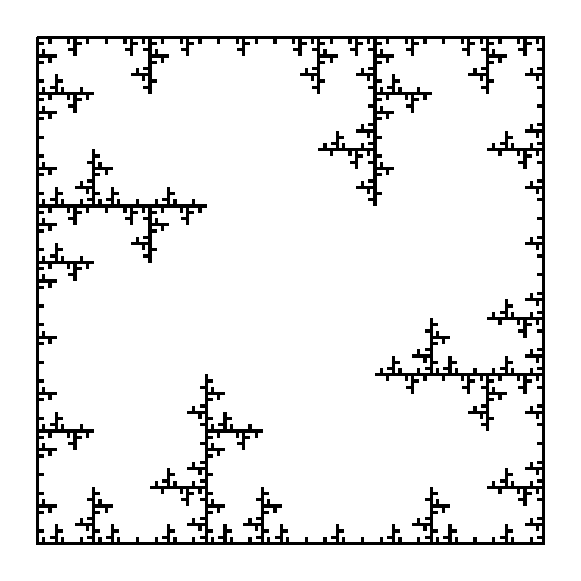
\includegraphics[width=8cm]{LSsystemKochd}}
\caption{Variation on Koch curve 4: n = 4, angle = 90, Input: \emph{F-F-F-F}, \emph{F $\rightarrow$ FF-F-\ -F-F}}
\label{fig:Kochd}
\end{figure}


\begin{tabbing}
\=aaa\=aaa\=aaaaaa\=aaaaaaaaa\=aaaaaaaaa\=aaaaaaaaa\=aaaaaaaaa\=aaaaaaaaa\=aaaaaaaaa\kill
Figure~\ref{fig:Kochd} with n=4 and \ref{fig:Koche} with n=5\\
\>\> \emph{Input} \>\>\emph{F-F-F-F}\\
\>\> \emph{Angle} \>\>90 degree\\
\>\> \emph{Rule}  \>\>\emph{F $\rightarrow$ FF-F-\ -F-F}
\end{tabbing}

\begin{figure}[!h]
\centerline{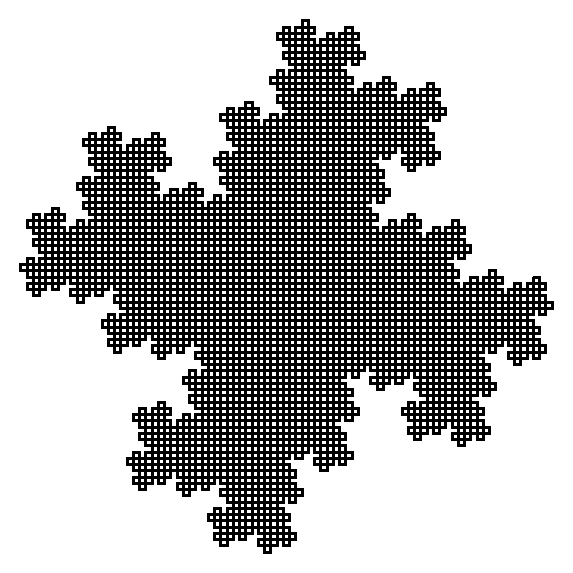
\includegraphics{LSsystemKoche}}
\caption{Variation on Koch curve 5: n = 5, angle = 90, Input: \emph{F-F-F-F}, \emph{F $\rightarrow$ F-FF--F-F}}
\label{fig:Koche}
\end{figure}







\begin{tabbing}
\=aaa\=aaa\=aaaaaa\=aaaaaaaaa\=aaaaaaaaa\=aaaaaaaaa\=aaaaaaaaa\=aaaaaaaaa\=aaaaaaaaa\kill
Figure~\ref{fig:Kochf} \\
\>\> \emph{Input} \>\>\emph{F-F-F-F}\\
\>\> \emph{Angle} \>\>90 degree\\
\>\> \emph{Rule}  \>\>\emph{F $\rightarrow$ F-F+F-F-F}
\end{tabbing}


\begin{figure}[!h]
\centerline{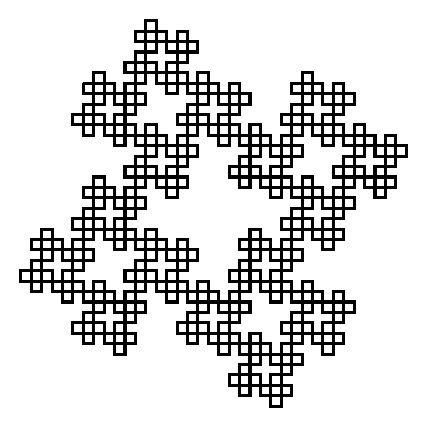
\includegraphics{LSsystemKochf}}
\caption{Variation on Koch curve 6: n = 4, angle = 90, Input: \emph{F-F-F-F}, \emph{F $\rightarrow$ F-F+F-F-F}}
\label{fig:Kochf}
\end{figure}



\section{Experimentation}

We suggest you to try the following L-Systems that we only describe here then try to create the L-System that produce the snow flakes shown in Figure~\ref{fig:snow}.

\begin{tabbing}
\=aaa\=aaa\=aaaaaa\=aaaaaaaaa\=aaaaaaaaa\=aaaaaaaaa\=aaaaaaaaa\=aaaaaaaaa\=aaaaaaaaa\kill
Interesting at level 2  \\
\>\> \emph{Input} \>\>\emph{F-F-F-F}\\
\>\> \emph{Angle} \>\>90 degree\\
\>\> \emph{Rule}  \>\> \emph{F $\rightarrow$ F+FF-FF-F-F+F+FF-F-F+F+FF+FF-F}
\end{tabbing}


\begin{tabbing}
\=aaa\=aaa\=aaaaaa\=aaaaaaaaa\=aaaaaaaaa\=aaaaaaaaa\=aaaaaaaaa\=aaaaaaaaa\=aaaaaaaaa\kill
Interesting at level 3 \\
\>\> \emph{Input} \>\>\emph{F}\\
\>\> \emph{Angle} \>\>90 degree\\
\>\> \emph{Rule}  \>\>\emph{F $\rightarrow$ F+F-F-F+F}
\end{tabbing}

\begin{figure}
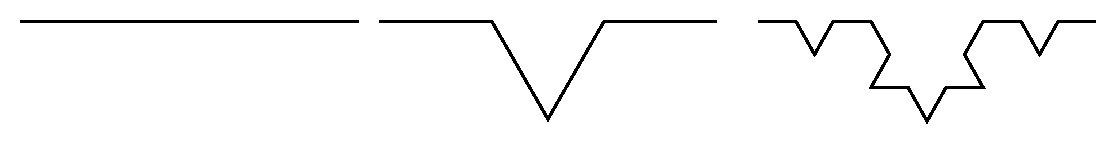
\includegraphics[width=\linewidth]{drawUnderTriangles}
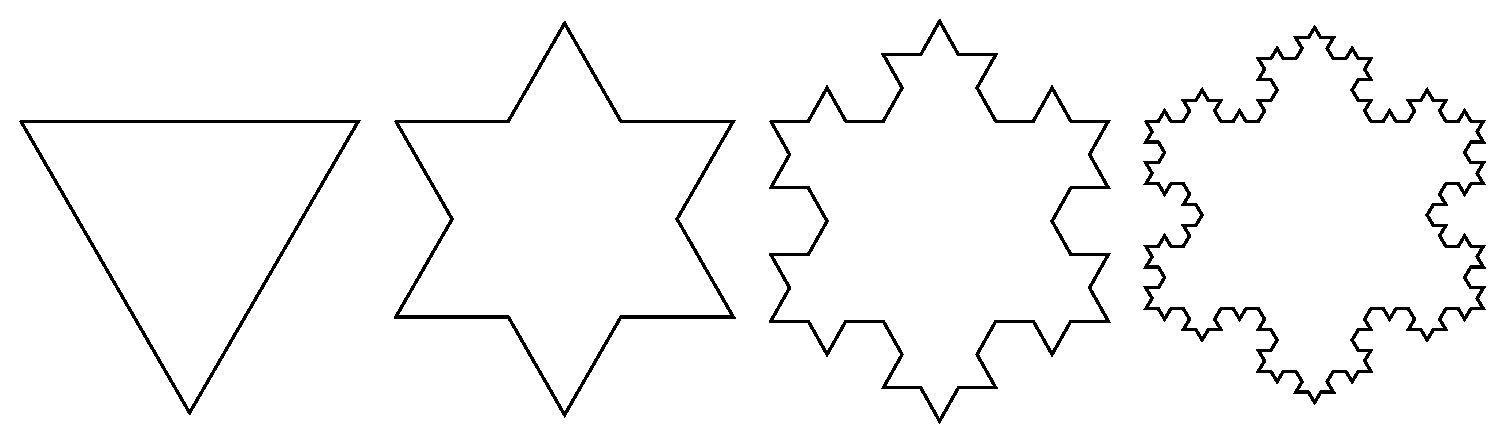
\includegraphics[width=\linewidth]{drawAllTriangle}
\caption{Steps to create a nice snow flake. \label{fig:snow}}
\end{figure}
\begin{exonofig}
Experiment and find the L-System generating the previous figures.
Hints: start with the smallest interesting input, the smallest level
of derivation and play with the production rule to generate the
transformation of a side.
\end{exonofig}

%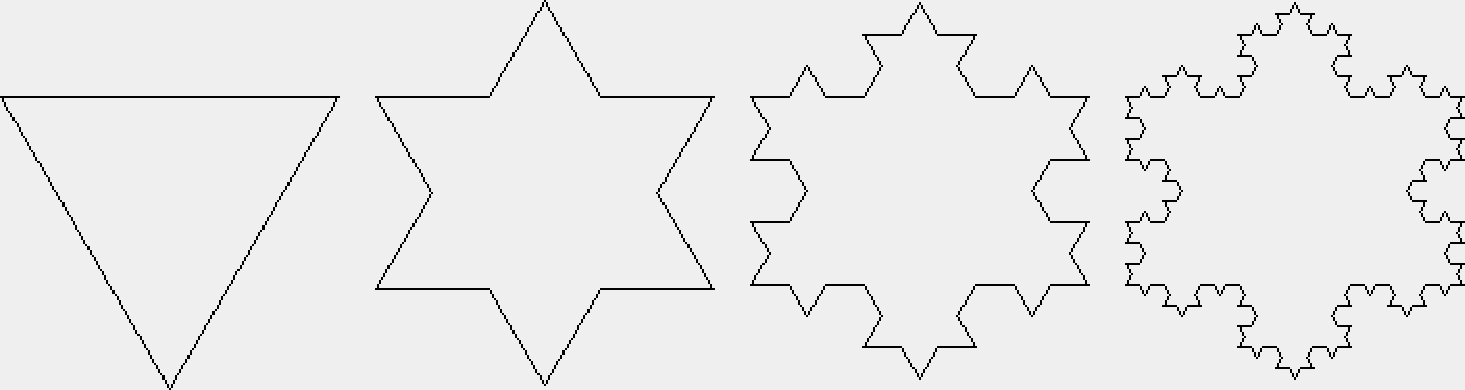
\includegraphics[width=\linewidth]{AllTriangles}
%\begin{exonofig}
%Experiment and find the L-System generating the previous figure.
%\end{exonofig}


\section{Analysis of the Solution}
The fact that the solution only allows the expression of single rule
L-System is not really a problem because we learnt this way the
essence of the problem and are now ready to develop a more complex
system.  From a methodological point of view this is a good
point. Some people think that producing the best solution handling all
kinds of variations is better, however often we cannot forsee
where the complex part will be and what are the possible variation. So having a small implementation up front working even in a limited setting is a way to understand the
problem. We should only be prepared to change it heavily or to simply
throw away what we made.


Even if the solution we proposed here is successful to manage trivial
L-Systems, its design is not really good bad from an object-oriented perspective. As this is not the topic of this book this is not really a problem. However, we just want to tell you why.
In fact methods should represent the behavior or responsibilities that an object is carrying. Here a method such as
\ct{interpret:length:angle:} clearly represents the behavior of a turtle. This method allow one to represent messages sent in another form, here strings.  But this is  not the case for the methods \ct{replace:by:in:} and \ct{applyOnInput:leftPart:rightPart:level:} 
that have nothing to do with a turtle. Second
these methods do not even use the state of the turtle or its
methods. This is a sign that they are defined in the wrong place. A good solution would define  a class representing an L-System and these methods would be moved there but this is the topic of another book. 


\ifx\wholebook\relax\else\end{document}\fi
